\section{Przechowywanie i eksport historii pozycji}
\label{sec:historia-eksport}

Aby umożliwić analizę zebranych danych pomiarowych, konieczne było zaimplementowanie mechanizmu
przechowywania historii pozycji węzłów oraz funkcji eksportu tych danych do formatu CSV.
Zaimplementowano cztery funkcjonalności: 
- mechanizm przechowywania historii pozycji węzłów i wyświetlania "śladu" na mapie
- eksport zebranych danych pozycji do pliku CSV, 
- eksport logu zdarzeń geofencingu (wejść i wyjść ze stref) 
- eksport definicji stref (geometrii wielokątów wraz z listą obserwowanych węzłów). 
Pierwsze dwie funkcjonalności mogą służyć użytkownikowi do wizualizacji ścieżki, którą poruszał się węzeł. Kolejne dwie funkcjonalności potrzebne są w większym stopniu do sprawdzenia dokładności, a co za tym idzie "przydatności" aplikacji i systemu. Eksport definicji stref umożliwia odtworzenie geometrii stref poza aplikacją - np. do naniesienia na mapę i obliczenia odległości wystąpienia zdarzenia WEJŚCIA/WYJŚCIA do/ze strefy od rzeczywistego miejsca przecięcia granicy strefy i ścieżki węzła. 

\subsection*{Przechowywanie historii pozycji}
\label{sec:historia}

\paragraph{Model danych.}

Pojedynczy punkt reprezentuje klasa \texttt{TimedPosition}:

\begin{lstlisting}[caption={Klasa \texttt{TimedPosition} - pojedynczy punkt},
                   label={lst:timed-position}]
data class TimedPosition(
    val latitude: Double,
    val longitude: Double,
    val altitude: Int,
    val timestampSeconds: Int,
    val snr: Float
    val rssi: Int
)
\end{lstlisting}

Stan przechowywany jest wyłącznie w~pamięci operacyjnej, dlatego restart aplikacji
powoduje utratę historii - jest to zachowanie celowe, ponieważ dane sesji pomiarowej
nie powinny wpływać na kolejne sesje.

\subsection*{Eksport danych sesji do CSV}
\label{sec:eksport-csv}

Eksportem zajmuje się \texttt{CsvExporter}, który zbiera dane z~\texttt{\seqsplit{PositionHistoryRepository}}
i~\texttt{\seqsplit{PacketStatsRepository}}, a~następnie zapisuje plik przez standardowy mechanizm \texttt{MediaStore.Downloads}. Nagłówek zawiera 16 kolumn zebranych w (tabli~\ref{tab:csv-kolumny}).

\begin{table}[!h]
    \caption{Kolumny pliku CSV}
    \label{tab:csv-kolumny}
    \centering
    \small
    \begin{tabular}{|p{3.2cm}|p{4.3cm}|p{5.5cm}|}
        \hline
        \textbf{Kolumna} & \textbf{Źródło} & \textbf{Uwagi} \\
        \hline
        \texttt{timestamp\_unix}    & \texttt{\seqsplit{TimedPosition.timestampSeconds}} & Czas GPS lub czas odbioru \\
        \texttt{\seqsplit{timestamp\_readable}}& j.w., sformatowany & \texttt{yyyy-MM-dd HH:mm:ss} \\
        \texttt{node\_id}           & \texttt{\seqsplit{MeshNodeInfo.getId()}} & np.\ \texttt{!a1b2c3d4} \\
        \texttt{node\_name}         & \texttt{\seqsplit{MeshNodeInfo.getDisplayName()}} & Snapshot z~chwili eksportu \\
        \texttt{role}               & \texttt{MeshUser.role} & CLIENT, TRACKER, ROUTER itd. \\
        \texttt{lat}, \texttt{lng}  & \texttt{TimedPosition} & 6 miejsc po przecinku \\
        \texttt{altitude\_m}        & \texttt{\seqsplit{TimedPosition.altitude}} &  \\
        \texttt{snr\_db}            & \texttt{MeshNodeInfo.snr} & Puste jeśli \texttt{Float.MAX\_VALUE} \\
        \texttt{rssi\_dbm}          & \texttt{MeshNodeInfo.rssi} & Puste jeśli \texttt{Int.MAX\_VALUE} \\
        \texttt{delta\_t\_s}        & \texttt{PacketStatsRepository} & $\Delta t$ od poprzedniego broadcastu \\
        \hline
    \end{tabular}
    \normalsize
\end{table}

Każdy punkt z~historii \texttt{PositionHistoryRepository} staje się jednym wierszem CSV.
Węzły bez historii pozycji (np.\ węzły wewnątrz budynku, bez fixa GPS) eksportowane są
jako jeden wiersz z~aktualnym stanem - kolumny \texttt{lat} i~\texttt{lng} pozostają
puste, natomiast dostępne metadane (SNR, RSSI, bateria) są wypełniane.

Jeśli historia jest pusta, metoda zwraca \texttt{Result.failure} z~komunikatem
\texttt{"empty"} i~plik nie jest tworzony.

\paragraph{Interfejs użytkownika.}

Eksport całej sesji dostępny jest w~sekcji ,,Dane testowe'' ekranu ustawień
(rysunek~\ref{fig:ustawienia-eksport}). Przycisk ,,Eksportuj sesję do CSV'' wywołuje
\texttt{\seqsplit{SettingsViewModel.exportSession()}}, który uruchamia \texttt{CsvExporter.export()}.
Po zakończeniu otwiera Android Share sheet z~gotowym plikiem. Przycisk ,,Wyczyść historię pozycji''
wywołuje \texttt{\seqsplit{positionHistoryRepository.clearAll()}} oraz
\texttt{\seqsplit{packetStatsRepository.resetAll()}} po potwierdzeniu przez \texttt{AlertDialog}.

\begin{figure}[h]
    \centering
    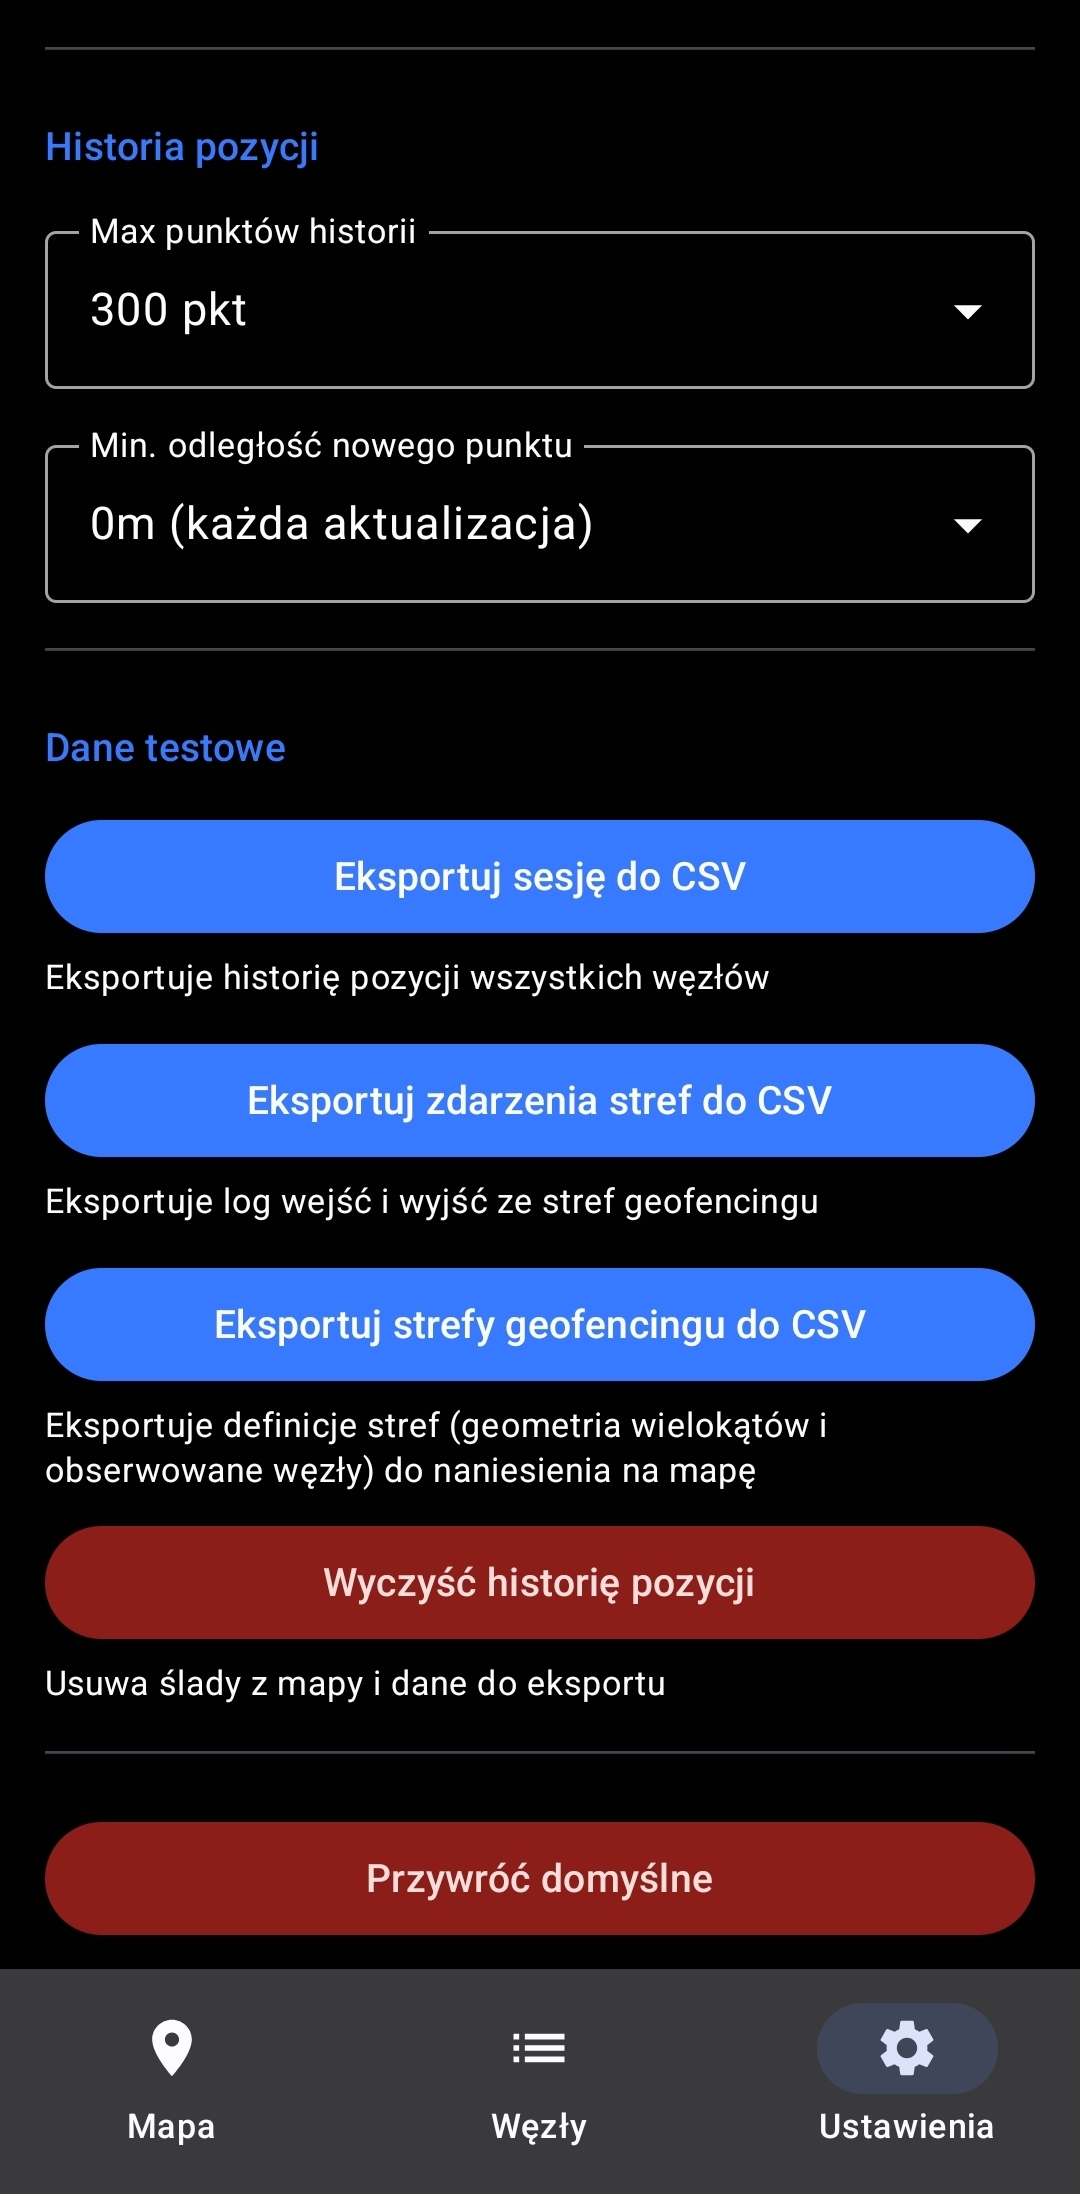
\includegraphics[width=0.45\linewidth]{img/ustawieniaEksport.jpg}
    \caption{Sekcja ,,Dane testowe'' w~ekranie ustawień aplikacji}
    \label{fig:ustawienia-eksport}
\end{figure}

\subsection*{Eksport zdarzeń geofencingu do CSV}
\label{sec:eksport-strefy}

Zdarzenia wejść i~wyjść ze stref (encja \texttt{ZoneEvent}, omówiona
w~rozdz.~\ref{sec:geofencing}) są przechowywane w~bazie Room i~nie są tracone po
restarcie aplikacji. Umożliwia to eksport pełnego logu zdarzeń z~całej sesji terenowej, nawet jeśli aplikacja była w~międzyczasie restartowana. Nazwa pliku przyjmuje format 
\texttt{meshtracker\_zones\_YYYYMMDD\_HHmmss.csv}, a plik zawiera 7 kolumn wymienionych w 

\begin{table}[!h]
    \caption{Kolumny pliku CSV zdarzeń stref}
    \label{tab:csv-strefy}
    \centering
    \small
    \begin{tabular}{|p{3.2cm}|p{4cm}|p{5cm}|}
        \hline
        \textbf{Kolumna} & \textbf{Źródło} & \textbf{Uwagi} \\
        \hline
        \texttt{timestamp\_unix}    & \texttt{\seqsplit{ZoneEvent.timestampSeconds}} & Czas rejestracji zdarzenia przez telefon \\
        \texttt{\seqsplit{timestamp\_readable}}& j.w., sformatowany & \texttt{yyyy-MM-dd HH:mm:ss} \\
        \texttt{zone\_id}           & \texttt{ZoneEvent.zoneId}           & UUID strefy \\
        \texttt{zone\_name}         & \texttt{Zone.name}                  & Nazwa nadana przez użytkownika \\
        \texttt{node\_id}           & \texttt{ZoneEvent.nodeId}           & Identyfikator węzła \\
        \texttt{node\_name}         & \texttt{\seqsplit{ZoneEvent.nodeName}}         & Snapshot nazwy z~chwili zdarzenia \\
        \texttt{event\_type}        & \texttt{\seqsplit{ZoneEvent.eventType}}        & \texttt{ENTER} lub \texttt{EXIT} \\
        \hline
    \end{tabular}
    \normalsize
\end{table}

Wiersze posortowane są rosnąco według znacznika czasu, co ułatwia obliczenie czasu
$T_z$ jako różnicy między fizycznym przekroczeniem granicy a~timestampem wiersza
\texttt{ENTER} lub \texttt{EXIT} w~arkuszu kalkulacyjnym.

\paragraph{Implementacja.}

Metoda \texttt{\seqsplit{CsvExporter.exportZoneEvents()}} pobiera zdarzenia ze wszystkich stref  -
zarówno aktywnych, jak i~dezaktywowanych  - ponieważ log historyczny nie powinien
zależeć od bieżącej konfiguracji monitoringu. Dostęp do bazy odbywa się przez dwa
jednorazowe zapytania DAO (\texttt{\seqsplit{getAllZonesOnce()}}, \texttt{\seqsplit{getEventsOnce(zoneId)}}),
a nie przez \texttt{Flow}, co jest właściwe w~kontekście \texttt{Dispatchers.IO}.

\paragraph{Interfejs użytkownika.}

W~sekcji ,,Dane testowe'' ekranu ustawień, poniżej przycisku ,,Eksportuj sesję do CSV'',
znajduje się przycisk ,,Eksportuj zdarzenia stref do CSV''. Wywołuje on
\texttt{\seqsplit{SettingsViewModel.exportZoneEvents()}}, a~wynik trafia do osobnego kanału
\texttt{\seqsplit{exportZonesEvent}}, obsługiwanego przez dedykowany \texttt{\seqsplit{LaunchedEffect}}
w~\texttt{SettingsScreen}. Jeśli baza nie zawiera żadnych zdarzeń, plik nie jest tworzony.

\subsection*{Eksport definicji stref geofencingu do CSV}
\label{sec:eksport-definicje-stref}

Trzeci wariant eksportu dotyczy samej \textbf{konfiguracji} stref -
geometrii wielokątów i~listy węzłów, które dana strefa monitoruje
tabela~\ref{tab:zone-entity}). W~odróżnieniu od eksportu zdarzeń (rozdz.~\ref{sec:eksport-strefy}),
który dokumentuje \emph{co się wydarzyło}, ten eksport dokumentuje \emph{jak zdefiniowano
strefę} - pozwala to np.\ odtworzyć granice stref w~zewnętrznym narzędziu GIS albo zachować
kopię zapasową konfiguracji przed jej modyfikacją lub usunięciem. Nazwa pliku przyjmuje format\\
\texttt{meshtracker\_zone\_definitions\_YYYYMMDD\_HHmmss.csv}.
Plik zawiera 8 kolumn (tabela~\ref{tab:csv-definicje-stref})

\begin{table}[!h]
    \caption{Kolumny pliku CSV definicji stref}
    \label{tab:csv-definicje-stref}
    \centering
    \small
    \begin{tabular}{|p{3cm}|p{3.7cm}|p{5.3cm}|}
        \hline
        \textbf{Kolumna} & \textbf{Źródło} & \textbf{Uwagi} \\
        \hline
        \texttt{zone\_id}            & \texttt{Zone.id}                          & UUID strefy \\
        \texttt{zone\_name}          & \texttt{Zone.name}                        & Nazwa nadana przez użytkownika \\
        \texttt{color\_argb}         & \texttt{\seqsplit{Zone.colorArgb}}        & Kolor strefy jako liczba ARGB \\
        \texttt{is\_active}          & \texttt{\seqsplit{Zone.isActive}}         & \texttt{true}/\texttt{false} \\
        \texttt{vertex\_index}       & Indeks w~liście wierzchołków              & Numeracja od 0 \\
        \texttt{vertex\_lat}, \texttt{vertex\_lon} & \texttt{\seqsplit{Zone.vertices()}} & 6 miejsc po przecinku \\
        \texttt{watched\_node\_ids}  & \texttt{\seqsplit{Zone.watchedNodeIds()}} & Lista ID węzłów rozdzielona średnikiem \texttt{;} \\
        \hline
    \end{tabular}
    \normalsize
\end{table}

Każdy wierzchołek wielokąta strefy staje się jednym wierszem CSV - dzięki temu plik
zachowuje pełną geometrię, kosztem denormalizacji (kolumny \texttt{zone\_id} .. \texttt{is\_active}
oraz \texttt{watched\_node\_ids} powtarzają się w~każdym wierszu należącym do tej samej
strefy). Jeżeli strefa nie posiada żadnych wierzchołków (przypadek brzegowy), eksportowany
jest pojedynczy wiersz z~pustymi kolumnami \texttt{vertex\_index}, \texttt{vertex\_lat}
i~\texttt{vertex\_lon}.

\paragraph{Implementacja.}

Metoda \texttt{\seqsplit{CsvExporter.exportZoneDefinitions()}} pobiera wszystkie strefy przez
\texttt{\seqsplit{zoneRepository.getAllZonesOnce()}} - zarówno aktywne, jak i~nieaktywne - a~następnie
dla każdej z~nich generuje wiersze na podstawie jej wierzchołków. Jeśli w~bazie nie ma
żadnej zdefiniowanej strefy, metoda zwraca \texttt{Result.failure} z~komunikatem
\texttt{"empty"} i~plik nie jest tworzony.

\paragraph{Interfejs użytkownika.}

W~sekcji ,,Dane testowe'' ekranu ustawień, poniżej przycisku ,,Eksportuj zdarzenia stref
do CSV'', znajduje się trzeci przycisk - ,,Eksportuj strefy geofencingu do CSV'', opisany
podpisem ,,Eksportuje definicje stref (geometria wielokątów i~obserwowane węzły) do
naniesienia na mapę'' (rysunek~\ref{fig:ustawienia-eksport}). Wywołuje on
\texttt{\seqsplit{SettingsViewModel.exportZoneDefinitions()}}, a~wynik trafia do osobnego
kanału \texttt{\seqsplit{exportZoneDefinitionsEvent}}, obsługiwanego przez dedykowany
\texttt{\seqsplit{LaunchedEffect}} w~\texttt{SettingsScreen}, który otwiera Android Share
sheet z~tytułem ,,Eksportuj strefy geofencingu''.
